\documentclass{beamer}

\usepackage[utf8]{inputenc}
\usepackage{tabularx}
\usepackage{amsmath}
\usepackage{amssymb}
\usepackage{booktabs}
\usepackage{centernot}
\usepackage{hyperref}
\usepackage{graphicx}
\usepackage{eufrak}
\usepackage{blindtext}
\graphicspath{{pics/}}

\usetheme{Frankfurt}

\title{Determinants}
\subtitle{Group 12}

\author{Catterwell, A. \quad Smith, M. \quad Wang, R. \quad Watson, K.}

\institute{University of Edinburgh}

\begin{document}

\begin{frame}
    \maketitle
\end{frame}

\begin{frame}{Overview}
    \tableofcontents
\end{frame}

\section{Using LU decomposition to compute determinants}

\subsection{What is LU decomposition?}

\begin{frame}{What is LU decomposition?}

    Somebody else do this section

    \begin{itemize}
        \item What LU decomposition is
        \item Its limitations
        \item How PLU decomposition addresses these limitations
    \end{itemize}

 \end{frame}

\subsection{Does it always work}

\begin{frame}{Does the LU decomposition always work}

    \textbf{Cases when the LU factorization exists.}

    \begin{itemize}
        \item A PLU factorization will always exist for a square matrix $A$.
        \item If a square matrix A is invertible and all its leading principal minors are nonzero,
            then a LU factorization will exist.
    \end{itemize}


\end{frame}

\begin{frame}{Does the LU decomposition always work (cont.)}

    \textbf{Cases where LU factorization will not always exist.}
    \begin{itemize}
        \item If $A$ is a singular matrix (i.e. $\det(A) = 0$), with $\text{rank}(A)=k$, we can't know for
            sure if the LU factorization will exist.

            \begin{itemize}
                \item If the first $k$ leading principal minors are non-zero, the LU factorization
                    exists.
                \item For an $n \times n$ matrix $A$ the LU factorization exists if
                    \[
                        \text{rank}(A_{1,1}) + n \geq \text{rank}
                        \begin{pmatrix}
                            A_{1,1} & A_{1,2}
                        \end{pmatrix}
                        + \text{rank}
                        \begin{pmatrix}
                            A_{1,1} \\ A_{2,1}
                        \end{pmatrix}
                    \]
            \end{itemize}

    \end{itemize}

\end{frame}

\begin{frame}{Does LU decomposition always work (cont.)}

    Simple example of when LU decomposition fails
    \[
        \begin{pmatrix}
            0 & 1\\ 1 & 0
        \end{pmatrix}
    \]

\end{frame}

\subsection{How it helps us compute determinants}

\begin{frame}{How it helps us compute determinants}

    We first start with $PA = LU$

    \begin{align*}
        A &= P^{-1}LU \\
          &= P^T LU
    \end{align*}

    since $P^{-1} = P^T$ by definition of an orthogonal matrix.

\end{frame}

\begin{frame}{How it helps us compute determinants (cont.)}

    Now we have $A=P^T LU$. So in a form where we can easily calculate the determinant.

    \begin{align*}
        \det(A) &= \det(P^T)\cdot\det(L)\cdot\det(U) \\
                &= \det(P)\cdot\det(L)\cdot\det(U)
    \end{align*}
    We can make this step as we know from algebra that,
    $\det(AB) = \det(A)\det(B)$ and also that $\det(A) = \det(A^T)$.

\end{frame}

\begin{frame}{How it helps us compute determinants (cont.)}

    Finally we have

    \[
        \det(A) = {(-1)}^s \left( \prod_{i=1}^{n} l_{i,i} \right)
        \left( \prod_{i=1}^{n} u_{i,i} \right)
    \]

    with $s$ being the number of row exchanges in the decomposition,
    which is the parity of the permutation matrix.

\end{frame}

\section{Other algorithms for computing determinants}

\subsection{Leibniz formula}

\begin{frame}{Leibniz formula}

    \begin{block}{Definition}
        The Leibniz formula defines the determinant of $A \in \mathbb{M}(n)$ as
        \[
            \det(A) = \sum_{\sigma \in \mathfrak{S}_n} \text{sgn}(\sigma)
            \prod_{i=1}^n a_{i,\sigma(i)}
        \]
        where $\mathfrak{S}_n$ is the set of permutations length $n$.
    \end{block}

    Computing the determinant using this method is slow with runtime $\mathcal{O}((N+1)!)$.

\end{frame}

\subsection{Laplace expansion}

\begin{frame}{Laplace expansion}

    The Laplace (1st row) expansion for computing determinants is usually the first method taught
    for computing determinants of $3 \times 3$ matrices and larger.

    \begin{block}{Theorem}
        The formula for the (1st row) Laplace expansion of $A \in \mathbb{M}(n)$
        is given as:
        \[
            \det(A) = \sum_{j=1}^n a_{1,j}\cdot C_{1,j}
        \]
        where $C_{i,j}$ is the $(i, j)$ cofactor of $A$.
    \end{block}

    Its runtime complexity of $\mathcal{O}(N!)$ is poor.

\end{frame}

\begin{frame}{Laplace expansion vs Leibniz formula}

    \begin{center}{}
        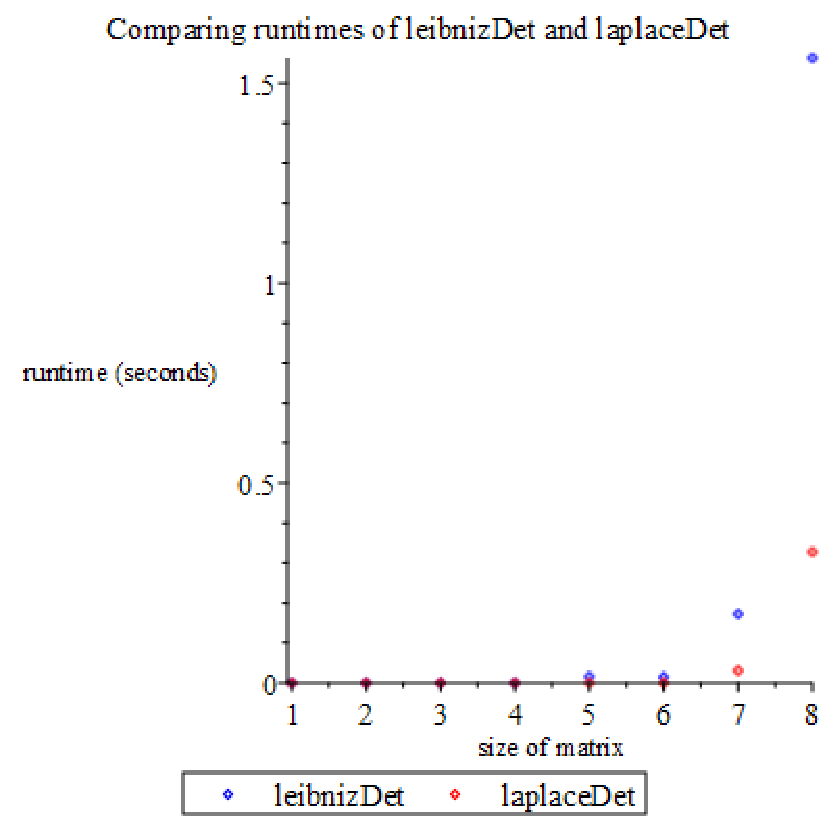
\includegraphics[height=180]{leibniz-laplace}
    \end{center}

    Runtimes are similar --- both run in exponential time.

\end{frame}

\begin{frame}{Laplace expansion vs LU decomposition}

    \begin{center}{}
        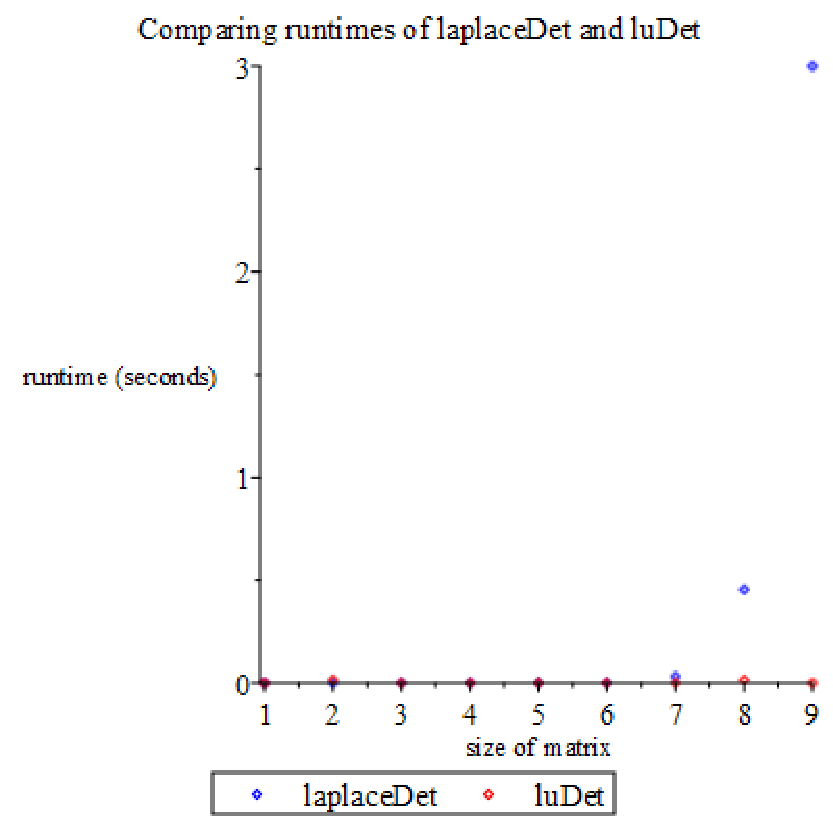
\includegraphics[height=180]{laplace-lu}
    \end{center}

    The difference between exponential and polynomial-time functions is clear.
    % Let's look at a better algorithm.
\end{frame}

\subsection{Gaussian elimination}

\begin{frame}{Gaussian elimination}

    \begin{itemize}

        \item The determinant of a triangular matrix can be computed by taking the product of its
            diagonal entries (which is a quick $\mathcal{O}(N)$ operation).

        \item Any invertible square matrix can be transformed into echelon form by performing
            Gaussian elimination, which takes $\mathcal{O}(N^3)$ time.

    \end{itemize}

    So how does it compare to LU decomposition?

\end{frame}

\begin{frame}{Gaussian elimination vs LU decomposition}

    \begin{center}{}
        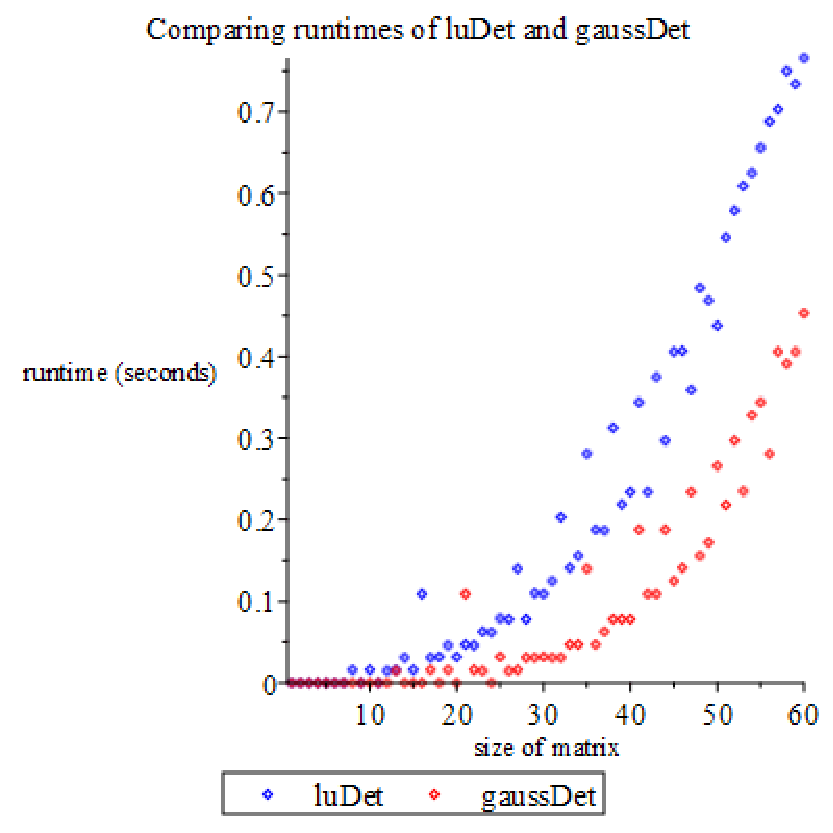
\includegraphics[height=180]{lu-gauss}
    \end{center}

    The difference in runtimes is small (a constant factor).
\end{frame}

\begin{frame}{Gaussian elimination (cont.)}

    Conventional Gaussian elimination requires division, meaning that solutions maybe inexact,
    so precision is lost.

    This is can be addressed by using\dots

\end{frame}

\subsection{Bareiss algorithm}

\begin{frame}{Bareiss algorithm}

    \begin{itemize}

        \item Addresses the issue of precision-loss by performing \emph{integer-preserving}
            Gaussian elimination on integer matrices.

        \item The runtime complexity is $\mathcal{O}(N^3)$ which is the same as conventional
            Gaussian Elimination, whilst preserving exactness.

            % TODO

    \end{itemize}

    % This is very complicated.  Are there any easier exact algorithms that run in polynomial time?

\end{frame}

\subsection{Bird's algorithm}

\begin{frame}{Bird's algorithm}

    Define $\mu : \mathbb{M}(n) \to \mathbb{M}(n)$:
    \[
        \mu(X) =
        \begin{pmatrix}{}
            \mu_{2,2} - x_{2,2} & x_{1,2}             & \cdots & x_{1,n-1}           & x_{1,n} \\
            0                   & \mu_{3,3} - x_{3,3} & \cdots & x_{2,n-1}           & x_{2,n} \\
            \vdots              & \vdots              & \ddots & \vdots              & \vdots \\
            0                   & 0                   & \cdots & \mu_{n,n} - x_{n,n} & x_{n-1,n} \\
            0                   & 0                   & \cdots & 0                   & 0
        \end{pmatrix}
    \]
    and $F_A : \mathbb{M}(n) \to \mathbb{M}(n)$,
    with $A \in \mathbb{M}(n)$
    \begin{align*}{}
        F_A(X)    & = \mu(X)\cdot A \\
        F_A^2(X)  & = \mu(F_A(X)) \cdot A \\
                  & \vdots \\
        F_A^n(X)  & = \mu(F_A^{n-1}(X)) \cdot A \\
    \end{align*}

\end{frame}

\begin{frame}{Bird's algorithm (cont.)}

    \begin{block}{Bird's Theorem}
        \[
            F_A^{n-1}(A) =
            \begin{pmatrix}{}
                d      & 0      & \cdots & 0 \\
                0      & 0      & \cdots & 0 \\
                \vdots & \vdots & \ddots & \vdots \\
                0      & 0      & 0      & 0
            \end{pmatrix}
            \text{with} \ d =
            \begin{cases}{}
                \det(A)  & \text{odd} \ n \\
                -\det(A) & \text{even} \ n \\
            \end{cases}
        \]
    \end{block}

    \begin{itemize}

        \item Enables the \emph{division-free} computation of determinants in
            $\mathcal{O}(n\cdot M(n))$ where $M(n)$ is the runtime complexity of the matrix
            multiplication algorithm used.

        \item If the conventional $\mathcal{O}(n^3)$ matrix multiplication algorithm is used,
            then Bird's algorithm will run in $\mathcal{O}(n^4)$ time.

        \item But this can be reduced to $\mathcal{O}(n^{3.8})$ by using the
            \emph{Strassen algorithm} for matrix multiplication.

    \end{itemize}

\end{frame}

\begin{frame}{Bird's algorithm vs LU decomposition}

    \begin{center}{}
        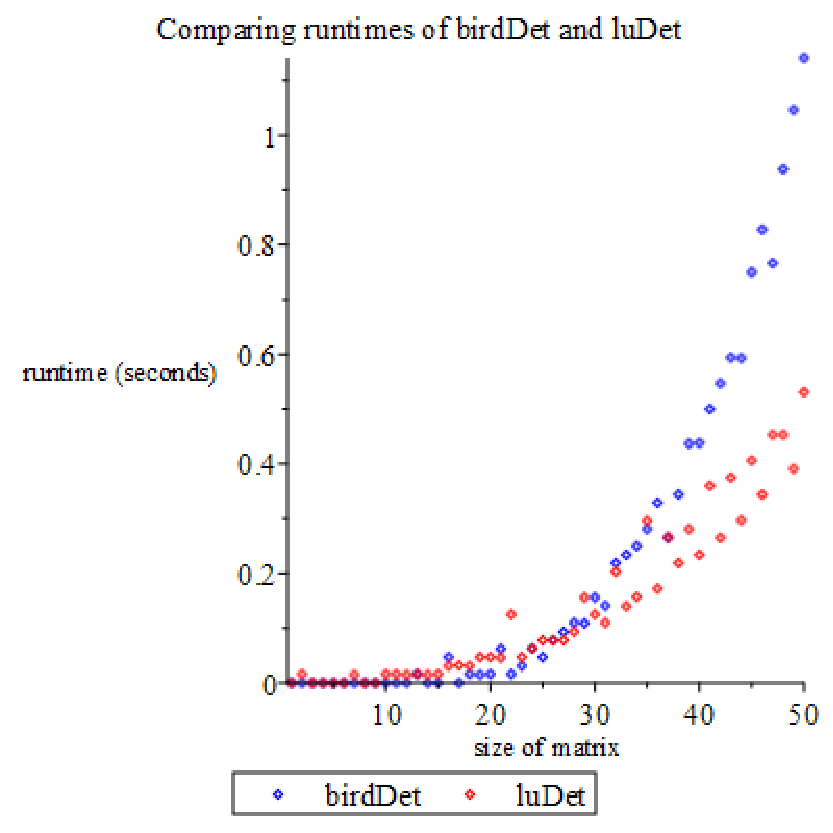
\includegraphics[height=180]{bird-lu}
    \end{center}

    Bird's runtimes increase noticeably more rapidly than LU decomposition,
    but it's still polynomial.

\end{frame}

\section{Epilogue}

\subsection{Summary of determinant algorithms}

\begin{frame}{Summary of determinant algorithms}

    \begin{center}
        \begin{tabular}{l l l}
            \toprule
            \emph{Algorithm}     & \emph{Runtime}           & \emph{Exact} \\
            \midrule
            Leibniz formula      & $\mathcal{O}((N+1)!)$    & Yes \\
            Laplace expansion    & $\mathcal{O}(N!)$        & Yes \\
            LU decomposition     & $\mathcal{O}(N^3)$       & No \\
            Gaussian elimination & $\mathcal{O}(N^3)$       & No \\
            Bareiss algorithm    & $\mathcal{O}(N^3)$       & Yes \\
            Bird's algorithm     & $\mathcal{O}(N^{3.8})$   & Yes \\
            \bottomrule
        \end{tabular}
    \end{center}

\end{frame}

\subsection{How fast is Maple's implementation?}

\begin{frame}{How fast is Maple's built-in determinant function?}

    \begin{center}{}
        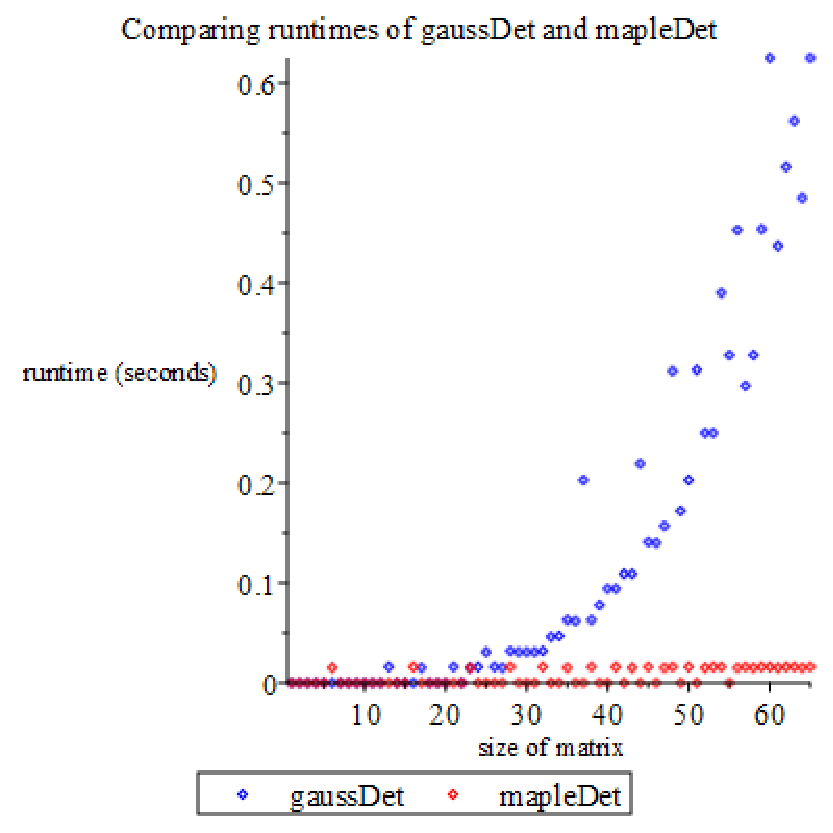
\includegraphics[height=180]{gauss-maple}
    \end{center}

    Very. Maple's optimisation means a fair comparison cannot be made.

\end{frame}

\begin{frame}

    \begin{center}
        \Huge{Thanks!}
    \end{center}

\end{frame}

\end{document}
